\begin{figure}[tbp]
\centering
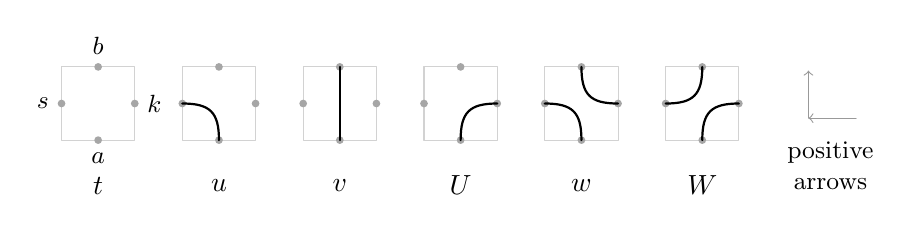
\begin{tikzpicture}[scale=.93,line cap=round,line join=round]
\foreach \j/\lab in {0/t,1/u,2/v,3/U,4/w,5/W} {
  \begin{scope}[shift={(1.65*\j,0)}]
  \draw[gray!35] (-.5,-.5) rectangle (.5,.5);
  \foreach \x/\y in {0/-.5,.5/0,0/.5,-.5/0}
    \fill[gray!70] (\x,\y) circle (1.5pt);
  \node at (0,-1.12) {$\lab$};
  \ifnum\j=0
    \node[below,font=\small] at (0,-.54) {$a$};
    \node[right,font=\small] at (.54,0) {$k$};
    \node[left,font=\small] at (-.54,0) {$s$};
    \node[above,font=\small] at (0,.54) {$b$};
  \fi
  \ifnum\j=1 \draw[thick] (0,-.5) .. controls (0,-.12) and (-.12,0) .. (-.5,0);\fi
  \ifnum\j=2 \draw[thick] (0,-.5)--(0,.5);\fi
  \ifnum\j=3 \draw[thick] (0,-.5) .. controls (0,-.12) and (.12,0) .. (.5,0);\fi
  \ifnum\j=4
    \draw[thick] (0,-.5) .. controls (0,-.12) and (-.12,0) .. (-.5,0);
    \draw[thick] (.5,0) .. controls (.12,0) and (0,.12) .. (0,.5);
  \fi
  \ifnum\j=5
    \draw[thick] (0,-.5) .. controls (0,-.12) and (.12,0) .. (.5,0);
    \draw[thick] (-.5,0) .. controls (-.12,0) and (0,.12) .. (0,.5);
  \fi
  \end{scope}
}
\begin{scope}[shift={(10,0)}]
  \draw[->,gray!80] (-.3,-.2)--(-.3,.45);
  \draw[->,gray!80] (.35,-.2)--(-.3,-.2);
  \node[font=\small,align=center] at (0,-.85) {positive\\arrows};
\end{scope}
\end{tikzpicture}
\caption{The six local connection weights in the row convention
\(B_{s,b;a,k}\). The first cell labels the bottom/right input ports
\(a,k\) and left/top output ports \(s,b\); positive arrows point upward
and leftward. A dot is a port; an unused port is vacant. For each
single-strand cell, its complementary pair of
ports has the same unoriented weight. Each strand may be oriented either
way, with the phase specified in the text. The two double-strand cells
are noncrossing.}
\label{a:local-cells}
\end{figure}
